\documentclass{beamer}

%%% Fichier de préambule avec toutes les définitions communes aux trois diaporamas

% Packages
\usepackage[utf8]{inputenc}  % Encodage : UTF-8
\usepackage[T1]{fontenc}     % Caractères français

\usepackage[french]{babel}   % Langue française

\usepackage{amsmath}         % Maths améliorées
\usepackage{amssymb}         % Symboles mathématiques
\usepackage{amsfonts}        % Polices mathématiques
\usepackage{graphicx}        % Inclusion d'images (PNG, GIF, PDF)
\usepackage{array}           % Tableaux améliorés
\usepackage[normalem]{ulem}  % Styles barré et souligné
\usepackage{listings, multicol, xcolor} % Listings (code source)
\usepackage{lmodern}         % Police d'écriture
\usepackage{url, hyperref}   % Liens hypertexte

\usepackage{tikz}            % TikZ : figures avancées
\usepackage{circuitikz}      % Circuits électriques en TikZ
% Diverses bibliothèques pour TikZ
\usetikzlibrary{chains, calc, decorations.pathmorphing, fadings, shadings, arrows, decorations.pathreplacing, shapes} 



% Commande \meta pour les listings
\newcommand{\meta}[1]{\ensuremath\langle\itshape#1\ensuremath\rangle}

% Paramètres des listings
\lstset{
upquote=false,
columns=flexible,
basicstyle=\ttfamily\scriptsize,
language={[LaTeX]TeX},
identifiersstyle=\color{green},
emphstyle=\color{blue},
keywordstyle=\color{blue},
directivestyle=\color{blue},
commentstyle=\color{gray},
    inputencoding=utf8,
literate={eacute}{\'e}1,    % Permet de faire des accents dans un listing avec £\'e£, £\`e£, £\`a£
    {eagrave}{\`e}1,
    {aagrave}{\`a}1,
    escapechar={£},
    moretexcs={meta},
morekeywords={              % Mots-clefs supplémentaires
  part,chapter,subsection,subsubsection,
  frontmatter,mainmatter,backmatter,
  tableofcontents,listoffigures,listoftables,titlepage,
  includegraphics,includepdf,
  dddot,ddddot,
  frametitle,framesubtitle,
  pause,only,uncover,
  usetheme,usecolortheme,
  institute,maketitle,
  usetikzlibrary,
  node,path,
  commande
}
}



% Thème Beamer
\usetheme{CambridgeUS}



% Auteurs et licence
\author[Folschette, Jubien, Tanguy]{Maxime \textsc{Folschette\up{1} } \and Anthony \textsc{Jubien\up{2}} \and Julien \textsc{Tanguy\up{3}} \\ 
{\scriptsize  \up{1} IRCCyN équipe MeForBio \\
\up{2} IRCCyN équipe Robotique et ONERA Toulouse \\
\up{3} IRCCyN équipe Systèmes Temps Réels \\
maxime.folschette, anthony.jubien, julien.tanguy @irccyn.ec-nantes.fr} }
\institute[AED]{Association des Étudiants en Doctorat de l'ECN (AED)  \\ 
Document sous licence Creative Commons BY 3.0 FR \\
http://creativecommons.org/licenses/by/3.0/fr/}



% Suppression des icônes de navigation
\setbeamertemplate{navigation symbols}{}

% Sommaire au début de chaque partie
\AtBeginPart{%
    \frame{\partpage}

    \begin{frame}
        \frametitle{Plan}
        \tableofcontents
    \end{frame}
}


\title[Séminaire \LaTeX, séance 2]{Séminaire \LaTeX, séance 2:\\ Documents scientifiques}
\date{mardi 18 février 2014}

\begin{document}

%%%%%%%%% SLIDE %%%%%%%%%%%%%%%%%%

\begin{frame}
    \titlepage
\end{frame}

%%%%%%%%% SLIDE %%%%%%%%%%%%%%%%%%

\begin{frame}{Points abordés durant la séance 2:}
    \begin{itemize}
            \item rappel de la dernière séance,
            \item présentation de commandes \LaTeX courantes,
            \item rédaction d'un document scientifique complet,
            \item présentation d'outils de gestion de la bibliographie. 
        \end{itemize}
\end{frame}

%%%%%%%%%%%%%%%%%%%%%%%%%%%%%%
%%%%%%%%%%% PART%% %%%%%%%%%%%%%%
%%%%%%%%%%%%%%%%%%%%%%%%%%%%%%

\part{Rappels}

%%%%%%%%%%%%%%%%%%%%%%%%%%%%%%
%%%%%%%%%%% SECTION %%%%%%%%%%%%%%
%%%%%%%%%%%%%%%%%%%%%%%%%%%%%%

\section{Rappel : Structure de base d'un document \LaTeX}

%%%%%%%%% SLIDE %%%%%%%%%%%%%%%%%%

\begin{frame}[fragile, label=latex-struct]
    \frametitle{Rappel: structure de base d'un document \LaTeX}
    \begin{itemize}
        \item Classe du document \lstinline|\documentclass{classe}|
        \item Préambule
        \item Corps du document, entre \lstinline|\begin{document}| et \lstinline|\end{document}|
    \end{itemize}

Le fichier source porte l'extension \texttt{.tex}. 

\end{frame}


%%%%%%%%% SLIDE %%%%%%%%%%%%%%%%%%

\begin{frame}[fragile]
    \frametitle{Des documents avec \texttt{class}}
    \begin{lstlisting}
        \documentclass[£\meta{option1}£, £\meta{option2}£, ...]{£\meta{classe}£}
    \end{lstlisting}
    \begin{block}{Classes de document}
        \begin{itemize}
            \item \textbf{article} ou \textbf{proc}: pour les publications,
            \item \textbf{report}: pour les thèses et rapports,
            \item \textbf{beamer}: pour les présentation,
            \item \textbf{book}, \textbf{letter}, \dots : il y a du choix!
        \end{itemize}
    \end{block}
    \begin{block}{Options de classe}
        \begin{itemize}
            \item \textbf{Xpt} : changer la taille des caractères
            \item \textbf{a4paper}: marges pour l'impression en A4
            \item \textbf{twoside}: impression recto-verso
        \end{itemize}
    \end{block}
\end{frame}

%%%%%%%%% SLIDE %%%%%%%%%%%%%%%%%%

\begin{frame}[fragile]
    \frametitle{Particularité de la classe \texttt{book}}
   
La classe \texttt{book} permet de distinguer les parties principales du document:
        \begin{itemize}
            \item \lstinline|\frontmatter| : introduction
            \item \lstinline|\mainmatter|: corps
            \item \lstinline|\backmatter|: annexes (insertion avec la commande  \lstinline|\appendix|)
        \end{itemize}

\end{frame}





%%%%%%%%% SLIDE %%%%%%%%%%%%%%%%%%

\section{Paquets} 

\begin{frame}[fragile]
    \frametitle{Rappel: de nombreux \texttt{packages}}
    \begin{lstlisting}
        \usepackage[£\meta{option1}£, £\meta{option2}£]{£\meta{paquet}£}
    \end{lstlisting}
    \begin{block}{Paquets usuels}
        \begin{lstlisting}[multicols=2]
% accents
\usepackage[latin1]{inputenc}
\usepackage[T1]{fontenc}
%formules mathematiques
\usepackage{amsmath}
\usepackage{amsfonts}
\usepackage{amssymb}
%inclusion de fichier pdf
\usepackage{pdfpages}
%positionnement des figures
\usepackage{float}
%document en francais
\usepackage[francais]{babel}
%divers
\usepackage[left,pagewise]{lineno}
\usepackage{graphicx}
\usepackage{array}
        \end{lstlisting}
    \end{block}
\end{frame}


%%%%%%%%%%%%%%%%%%%%%%%%%%%%%%
%%%%%%%%%%% SECTION %%%%%%%%%%%%%%
%%%%%%%%%%%%%%%%%%%%%%%%%%%%%%

\section{Chapitres, sections, sous-sections}

%%%%%%%%% SLIDE %%%%%%%%%%%%%%%%%%

\begin{frame}[fragile]
\frametitle{Rappel: chapitres, sections, sous-sections...}


Les commandes sont en début de chaque découpage
\begin{itemize}
\item\lstinline?\part{titre}?: partie
\item\lstinline?\chapter{titre}?: chapitre (uniquement pour les classes \texttt{report} et \texttt{book})
\item\lstinline?\section{titre}?: section
\item\lstinline?\subsection{titre}?: sous-section
\item\lstinline?\subsubsection{titre}?: sous-sous-section
\end{itemize}

\medskip
Une ligne vide permet de commencer un nouveau paragraphe. Exemple :

\begin{columns}
  \begin{column}{0.40\textwidth}
\begin{lstlisting}
| Voici mon premier paragraphe.
|
| Et le second paragraphe
| qui est sur plusieurs 
| lignes.
\end{lstlisting}
  \end{column}
  \begin{column}{0.55\textwidth}
\rmfamily
Voici mon premier paragraphe.

Et le second paragraphe
qui est sur plusieurs
lignes.
  \end{column}
\end{columns}
  
\end{frame}

%%%%%%%%% SLIDE %%%%%%%%%%%%%%%%%%

\begin{frame}[fragile]
\frametitle{Rappel: chapitres, sections, sous-sections...}

Insertion d'une table des matières avec le commande \lstinline?\tableofcontents?.

\vspace*{3mm}

Pour éviter la numérotation et l'indexation dans la table des matières:

\lstinline?\section*{titre}?

\vspace*{3mm}

Pour éviter la numérotation mais forcer l'indexation dans la table des matières:

\lstinline?\section*{titre}?

\lstinline?\addcontentsline{toc}{section}{titre}?

\end{frame}




%%%%%%%%% SLIDE %%%%%%%%%%%%%%%%%%

\begin{frame}[fragile]
\frametitle{Exercice}

    \begin{lstlisting}[title={\texttt{exercice.tex}}]
        \documentclass[a4paper]{article}
        \usepackage[utf8]{inputenc}
        \usepackage[T1]{fontenc}
        \usepackage[french]{babel}
        \author{Preacutenom Nom}
        \title{Le titre}
        \date{\today}

        \begin{document}
        \maketitle

        ...

        \end{document}
    \end{lstlisting}

\end{frame}


%%%%%%%%% SLIDE %%%%%%%%%%%%%%%%%%

\begin{frame}[fragile]
\frametitle{Exercice}

    \begin{lstlisting}[title={\texttt{exercice.tex}}]

        \tableofcontents

        \section{titre1}
        ...

        \subsection{titre2}
        ...

        \section*{titre3}
        \addcontentsline{toc}{section}{titre3}
        ...


    \end{lstlisting}

\end{frame}


%%%%%%%%%%%%%%%%%%%%%%%%%%%%%%
%%%%%%%%%%% PART%% %%%%%%%%%%%%%%
%%%%%%%%%%%%%%%%%%%%%%%%%%%%%%

\part{Inclusion}

%%%%%%%%%%%%%%%%%%%%%%%%%%%%%%
%%%%%%%%%%% SECTION %%%%%%%%%%%%%%
%%%%%%%%%%%%%%%%%%%%%%%%%%%%%%

\section{Commande d'insertion}

%%%%%%%%%% SLIDE %%%%%%%%%%%%%%%%%%

\begin{frame}[fragile]
\frametitle{Rappel: commande d'insertion}

\begin{itemize}
\item\lstinline?\titlepage?: insère la page de titre
\item\lstinline?\clearpage?: insère un saut de page (1 maximum)
\item\lstinline?\newpage?: insère une nouvelle page
\item\lstinline?\cleardoublepage?: insère un saut de page sur page impaire
\item\lstinline?\tableofcontents?: insère une table des matières
\item\lstinline?\listoffigures?: insère une table des figures (séance 2)
\item\lstinline?\listoftables?: insère une table des tableaux (séance 2)
\item \dots
\end{itemize}

\end{frame}

%%%%%%%%%%%%%%%%%%%%%%%%%%%%%%
%%%%%%%%%%% SECTION %%%%%%%%%%%%%%
%%%%%%%%%%%%%%%%%%%%%%%%%%%%%%

\section{Inclusion de fichier .tex}

%%%%%%%%%% SLIDE %%%%%%%%%%%%%%%%%%

\begin{frame}[fragile]
\frametitle{Inclusion de fichier .tex}

Intérêt? simplifier l'écriture de fichiers \LaTeX{} importants en les découpant. 

Impératif: les fichiers-esclaves doivent être dans le même répertoire que le fichier-maître. 

\vspace*{3mm}

Commande: 

\lstinline?\input{fichier1}? pour inclure \lstinline?fichier1.tex? à l'emplacement désiré. 

\end{frame}


%%%%%%%%% SLIDE %%%%%%%%%%%%%%%%%%

\begin{frame}[fragile]
\frametitle{Exercice}

    \begin{lstlisting}[title={\texttt{exercice.tex}}]

        \input{monfichier1} %texte 1 
        \input{monfichier2} %texte 2
        \input{monfichier3} %texte 3

    \end{lstlisting}

\end{frame}

%%%%%%%%%%%%%%%%%%%%%%%%%%%%%%
%%%%%%%%%%% SECTION %%%%%%%%%%%%%%
%%%%%%%%%%%%%%%%%%%%%%%%%%%%%%

\section{Inclusion}

%%%%%%%%%% SLIDE %%%%%%%%%%%%%%%%%%

\begin{frame}[fragile]
\frametitle{Inclusion d'image simple}

Commande: 

\lstinline?\includegraphics{nomdufichier}? pour insérer l'image à l'emplacement considéré. 

\vspace*{3mm}

Pour une image placée dans sous-répertoire:

\lstinline?\includegraphics{nomsousrepertoire/nomdufichier}? 

\vspace*{3mm}

\begin{itemize}
\item Permet d'insérer une image (format: jpg, gif, pdf\dots.)  simplement,
\item inutile de préciser l'extension du fichier,
\item cette commande est rarement utilisée seule (voir suite).
\end{itemize}

\end{frame}

%%%%%%%%%% SLIDE %%%%%%%%%%%%%%%%%%

\begin{frame}[fragile]
\frametitle{Inclusion de fichier pdf}

Commande: 

\lstinline?\includepdf[pages=-]{nomdufichier}? pour insérer toutes les pages d'un pdf.

\vspace*{3mm}

\lstinline?\includepdf[pages={3,5-8,60,80}]{nomdufichier}? pour insérer seulement certaines pages d'un pdf.

\vspace*{3mm}

\begin{itemize}
\item Très pratique pour inclure des gros documents pdf (page(s) A4...),
\item préférer la commande \lstinline?\includegraphics{nomdufichier}? pour un graphique en pdf.
\end{itemize}

\end{frame}

%%%%%%%%% SLIDE %%%%%%%%%%%%%%%%%%

\begin{frame}[fragile]
\frametitle{Exercice}

    \begin{lstlisting}[title={\texttt{exercice.tex}}]

\includepdf[pages=-]{nomdufichier} %fichier pdf entier

    \end{lstlisting}

\end{frame}



%%%%%%%%%%%%%%%%%%%%%%%%%%%%%%
%%%%%%%%%%% PART%% %%%%%%%%%%%%%%
%%%%%%%%%%%%%%%%%%%%%%%%%%%%%%

\part{Environnements et environnement figure}

%%%%%%%%%%%%%%%%%%%%%%%%%%%%%%
%%%%%%%%%%% SECTION %%%%%%%%%%%%%%
%%%%%%%%%%%%%%%%%%%%%%%%%%%%%%

%%%%%%%%% SLIDE %%%%%%%%%%%%%%%%

\section{Commandes}

\begin{frame}[fragile]
\frametitle{Environnement}

\begin{lstlisting}
\begin{£\meta{nom-environnement}£}    % Debut de l'environnement
  ...
  ...   % Contenu de l'environnement
  ...
\end{£\meta{nom-environnement}£}      % Fin de l'environnement
\end{lstlisting}

\vspace*{3mm}
Permet de définir le début de la fin d'un environnement (figures, équations mathématiques, etc.).

Un environnement peut être inclus dans un autre (de même type ou non).

\end{frame}

%%%%%%%%%%%%%%%%%%%%%%%%%%%%%%
%%%%%%%%%%% SECTION %%%%%%%%%%%%%%
%%%%%%%%%%%%%%%%%%%%%%%%%%%%%%

\section{Environnement équation}

%%%%%%%%% SLIDE %%%%%%%%%%%%%%%%%%

\begin{frame}[fragile]
\frametitle{Environnement équation}

\begin{lstlisting}
\begin{equation} 
  1+1=0 
\end{equation} 
\end{lstlisting}

Permet d'insérer une équation mathématique numérotée (\ref{titre_eq}) :

\begin{equation} 
1+1=0 
\label{titre_eq} 
\end{equation} 

\end{frame}

%%%%%%%%% SLIDE %%%%%%%%%%%%%%%%%%

\begin{frame}[fragile]
\frametitle{Exercice}

\begin{lstlisting}[title={\texttt{exercice.tex}}]
\begin{equation} 
  2+3=5 
\end{equation} 
\end{lstlisting}

\end{frame}


%%%%%%%%% SLIDE %%%%%%%%%%%%%%%%%%

\begin{frame}[fragile]
\frametitle{Environnement itemize}

% Note : £\`e£ permet d'afficher un accent grave en mode listing (code source)
\begin{lstlisting}
\begin{itemize} 
  \item premi£\`e£re puce,
  \item deuxi£\`e£me puce,
  \item ...
\end{itemize} 
\end{lstlisting}

Permet d'insérer une liste à puces comme celle-ci:

\begin{itemize} %debut de l'environnement itemize
  \item première puce,
  \item deuxième puce,
  \item ...
\end{itemize} %fin de l'environnement itemize

\end{frame}

\begin{frame}[fragile]
\frametitle{Exercice}

\begin{lstlisting}[title={\texttt{exercice.tex}}]
\begin{itemize} 
  \item texte ligne 1 
  \item texte ligne 2 
  \item texte ligne 3 
  \item texte ligne 4 
\end{itemize} 
\end{lstlisting}

\end{frame}


%%%%%%%%%%%%%%%%%%%%%%%%%%%%%%
%%%%%%%%%%% SECTION %%%%%%%%%%%%%%
%%%%%%%%%%%%%%%%%%%%%%%%%%%%%%

\section{Environnement figure}

%%%%%%%%% SLIDE %%%%%%%%%%%%%%%%%%

\begin{frame}[fragile]
\frametitle{Environnement figure}

\begin{lstlisting}
\begin{figure}
  ...
\end{figure}
\end{lstlisting}

\vspace*{3mm}
L'environnement \texttt{figure} est un flottant:
\begin{itemize}
\item permet d'optimiser l'arrangement entre l'objet inséré et le reste du texte,
\item arrangement totalement automatique de la part de \LaTeX.
\end{itemize}

\end{frame}

%%%%%%%%% SLIDE %%%%%%%%%%%%%%%%%%

\begin{frame}[fragile]
\frametitle{Principe du flottant}

Possibilité de choisir le paramètre de position de l'objet inséré:

\begin{lstlisting}
\begin{figure}[position]
  ...
\end{figure}
\end{lstlisting}

\medskip
Choix de “position” parmi :
\begin{itemize}
\item \texttt{h} :  l'objet est inséré à l'emplacement considéré (déconseillé),
\item \texttt{t} : l'objet est inséré en haut de la page,
\item \texttt{b}  : l'objet est inséré en bas de la page,
\item \texttt{p} : l'objet est inséré sur une page réservée aux flottants (peu utilisé).
\end{itemize}

\medskip

On peut choisir plusieurs positions, la première est prioritaire :

\lstinline?\begin{figure}[ht]? (conseillé)

\medskip
“\texttt{!}” permet de passer outre les paramètres de placement de \LaTeX{} :

\lstinline?\begin{figure}[!h]? (déconseillé)

\end{frame}



%%%%%%%%% SLIDE %%%%%%%%%%%%%%%%%%

\begin{frame}[fragile]
\frametitle{Utilisation}

Utilisation la plus courante:

\vspace*{3mm}

\begin{lstlisting}
\begin{figure} 
  \centering 
  \includegraphics[£\meta{option}£]{£\meta{nom\_image}£} 
\end{figure} 
\end{lstlisting}

\vspace*{3mm}

\begin{itemize}
  \item Affiche une image centrée (commande \lstinline?\centering?),
  \item L'option de \lstinline?\includegraphics? permet de régler la taille de l'image :
  \begin{itemize}
    \item \lstinline?width=largeur en cm? ou
    \item \lstinline?height=hauteur en cm? ou
    \item \lstinline?scale=echelle? (1, 2, 0.5, ...)
  \end{itemize}
\end{itemize}

\end{frame}

%%%%%%%%% SLIDE %%%%%%%%%%%%%%%%%%

\begin{frame}[fragile]
\frametitle{Légende et étiquette}

Utilisation la plus courante:

\vspace*{3mm}

\begin{lstlisting}
\begin{figure} 
  \centering 
  \includegraphics[option]{nom_image} 
  \caption{legende}
  \label{etiquette}
\end{figure} 
\end{lstlisting}

\vspace*{3mm}

\begin{itemize}
\item  \lstinline?\caption{legende}?   permet d'insérer une légende à l'objet,
\item  \lstinline?\label{etiquette}?    ajoute une étiquette à l'objet. On pourra la référencer avec les commandes \lstinline?\ref{etiquette}? (numéro de figure) et \lstinline?\pageref{etiquette}? (numéro de page).
\end{itemize}

Exemple : cf. diapo \pageref{etiquette11}

\end{frame}

%%%%%%%%% SLIDE %%%%%%%%%%%%%%%%%%

\begin{frame}[fragile]
\frametitle{Exemple}

\vspace*{3mm}

\begin{figure} 
  \centering 
  
\includegraphics[width=9cm]{img/latex} 
  \caption{Logo \LaTeX}
  \label{etiquette11}
\end{figure} 

\end{frame}

%%%%%%%%% SLIDE %%%%%%%%%%%%%%%%%%

\begin{frame}[fragile]
\frametitle{Exercice}

Insérer une image, tester les options h, t, b.  Faire référence à cette image dans un paragraphe avec la commande \lstinline?\ref{etiquette1}?.

\begin{lstlisting}[title={\texttt{exercice.tex}}]
% Inclusion de la figure
\begin{figure}[t] 
  \centering 
  \includegraphics[width=5cm]{chemin-image} 
  \caption{titre}
  \label{etiquette1}
\end{figure} 

Comme on peut le voir £\`a£ la figure xxx, ...
% Faire une reference vers etiquette1
\end{lstlisting}

\end{frame}



%%%%%%%%%%%%%%%%%%%%%%%%%%%%%%
%%%%%%%%%%% PART%% %%%%%%%%%%%%%%
%%%%%%%%%%%%%%%%%%%%%%%%%%%%%%

\part{Equations mathématiques}


\section{Équations mathématiques}

%%%%%%%%% SLIDE %%%%%%%%%%%%%%%%%%

\begin{frame}[fragile]
\frametitle{Mathématiques sous LaTeX}

\begin{itemize}
\item \sout{éditeur d'équation nécessaire}
\item\sout{souris}
\item nécessité de connaitre les commandes usuelles
\item possibilité d'insérer des équation dans du texte:\\
  % Note : \rm et \rmfamily ne servent qu'à changer le type de police
  {\rmfamily blabla $\rm 1+1=4$ blabla}
\item possibilité d'insérer des équations entre deux paragraphes et de les numéroter automatiquement:
\end{itemize}

\begin{equation}
\rm 1+1=4
\end{equation}

\end{frame}

%%%%%%%%% SLIDE %%%%%%%%%%%%%%%%%%

\begin{frame}[fragile]
\frametitle{Équation ou notation mathématique dans le texte}

\begin{lstlisting}
blabla $\pi^2$ blabla $\sqrt{1+1}=0$ blabla
\end{lstlisting}

donne :

\medskip
\quad
blabla $\pi^2$ blabla $\sqrt{1+1}=0$ blabla

\medskip
Ou, selon la police du document :

\medskip
{\rmfamily\quad
blabla $\rm \pi^2$ blabla $\rm \sqrt{1+1}=0$ blabla
}
\end{frame}

%%%%%%%%% SLIDE %%%%%%%%%%%%%%%%%%

\begin{frame}[fragile]
\frametitle{Exercice}

Insérer plusieurs équations mathématique dans le texte, observer la typographie. 

\begin{lstlisting}[title={\texttt{exercice.tex}}]
texte $1+1=2$ texte
texte texte texte texte texte
texte texte  $1+1=2$...  
\end{lstlisting}

\end{frame}

%%%%%%%%% SLIDE %%%%%%%%%%%%%%%%%%

\begin{frame}[fragile]
\frametitle{Environnement équation }

\begin{lstlisting}
\begin{equation}       % debut de l'environnement equation
  1+1=0                % equation
  \label{titre_eq}     % etiquette de l'equation
\end{equation}         % fin de l'environnement equation
\end{lstlisting}

donne:

\begin{equation}
  1+1=0
  \label{titre_eq}
\end{equation}

\medskip
On peut utiliser l'étiquette de l'équation (\lstinline?titre_eq?) pour y faire référence :

\medskip
\begin{columns}
  \begin{column}{0.45\textwidth}
\begin{lstlisting}
Voir £\'e£quation (\ref{titre_eq}).
\end{lstlisting}
  \end{column}
  \begin{column}{0.45\textwidth}
\rmfamily
Voir équation (\ref{titre_eq}).
  \end{column}
\end{columns}

\end{frame}

%%%%%%%%% SLIDE %%%%%%%%%%%%%%%%%%

\begin{frame}[fragile]
\frametitle{Commandes usuelles 1}

\begin{itemize}
\item\lstinline?\sqrt{1+2}?: racine carrée $\Longrightarrow \sqrt{1+2}$
\item\lstinline?\sqrt[3]{1+2}?: racine carrée n-ième $ \Longrightarrow \sqrt[3]{1+2}$
\item\lstinline?\frac{1}{2}?: fraction $\Longrightarrow \frac{1}{2}$
\item\lstinline?\sin (1+2)?: cosinus $\Longrightarrow\sin (1+2)$
\item\lstinline?\cos (1+2)?: sinus $\Longrightarrow \cos (1+2)$
\item\lstinline?1^{1+2} ou 1^2?: puissance $\Longrightarrow 1^{1+2}$ ou $1^2$
\item\lstinline?1_{1+2} ou 1_2?: indice $\Longrightarrow1_{1+2}$ ou $1_2$
\item\lstinline?1_{1+2}^{1+3} ou 1_2^3?: puissance ET indice $\Longrightarrow 1_{1+2}^{1+3}$ ou $1_2^3$
\end{itemize}
\end{frame}



%%%%%%%%%%
\begin{frame}[fragile]
\frametitle{Commandes usuelles 2}

\begin{itemize}
\item \lstinline? \dot{v} \ddot{v} \dddot{v} \ddddot{v}?: dérivée $ \dot{v}$ $\ddot{v}$ $\dddot{v}$ $\ddddot{v}$
\item \lstinline? \vec{AB}?: vecteur $\vec{AB}$
\item \lstinline? \overline{1+i}?: conjugué $ \overline{1+i} $
\item \lstinline? \sum_a^b ?: somme $ \sum_a^b x$
\item \lstinline? \int_a^b ?: intégrale $ \int_a^b y$
\item \lstinline? \widehat {ABC}?: angle $ \widehat {ABC}$
\item \lstinline? 1+1 \mbox{ idem que } 1+1?: texte $ 1+1 \mbox{ idem que } 1+1$
\item \lstinline? \left( \frac{1}{2} \right) ?: parenthèse $ \left( \frac{1}{2} \right)$
\end{itemize}

Note : différents rendus selon la position.
\begin{equation}
\sum_a^b x \quad ; \quad \int_a^b y
\end{equation}

\end{frame}

%%%%%%%%% SLIDE %%%%%%%%%%%%%%%%%%

\begin{frame}[fragile]
\frametitle{Commandes usuelles 3}

\begin{itemize}
\item \lstinline? \begin{pmatrix} 1 & 2 \\ 3 & 4 \end{pmatrix}?: matrice type 'p' $ \begin{pmatrix} 1 & 2 \\ 3 & 4 \end{pmatrix}$
\item \lstinline? \begin{bmatrix} 1 & 2 \\ 3 & 4 \end{bmatrix}?: matrice type 'b' $ \begin{bmatrix} 1 & 2 \\ 3 & 4 \end{bmatrix}$
\item \lstinline? \begin{Bmatrix} 1 & 2 \\ 3 & 4 \end{Bmatrix}?: matrice type 'B' $ \begin{Bmatrix} 1 & 2 \\ 3 & 4 \end{Bmatrix}$
\item \lstinline? \begin{vmatrix} 1 & 2 \\ 3 & 4 \end{vmatrix}?: matrice type 'v' $ \begin{vmatrix} 1 & 2 \\ 3 & 4 \end{vmatrix}$
\item \lstinline? \begin{Vmatrix} 1 & 2 \\ 3 & 4 \end{Vmatrix}?: matrice type 'V' $ \begin{Vmatrix} 1 & 2 \\ 3 & 4 \end{Vmatrix}$
\end{itemize}


\end{frame}

%%%%%%%%%%
\begin{frame}[fragile]
\frametitle{Caractère grec}

\begin{itemize}
  \item Idée: nom de la lettre grecque
  \begin{itemize}
    \item “Nom” : Lettre majuscule,
    \item “nom”: lettre minuscule
  \end{itemize}
\end{itemize}

Exemples:

\lstinline?\Lambda?: donne $\Lambda$

\lstinline?\lambda?: donne $\lambda$
\end{frame}


%%%%%%%%%%
\begin{frame}[fragile]
\frametitle{Exemple d'équation complexe}

\begin{lstlisting}
A= \left(
\sqrt{\sum_{k=0}^{1000} \overline{5 k+i} }
\begin{bmatrix}
  1 & 2 & a \\
  3 & 4 & b \\
  5 & 6 & c \\
  7 & 8 & d
\end{bmatrix}
\frac{1+3+9+o+\frac{1}{2}} {n-m-\lambda}
\right)
\end{lstlisting}

donne:
\begin{equation} %début de l'environnement équation
A= \left(
\sqrt{\sum_{k=0}^{1000} \overline{5 k+i} }
\begin{bmatrix} 1 & 2 & a \\ 3 & 4 & b \\ 5 & 6 & c \\ 7 & 8 & d\end{bmatrix}
\frac{1+3+9+o+\frac{1}{2}} {n-m-\lambda}
\right)
\label{titre_éq} %label de l'équation (ex voir équation W)
\end{equation} %fin de l'environnement équation

\end{frame}

%%%%%%%%% SLIDE %%%%%%%%%%%%%%%%%%

\begin{frame}[fragile]
\frametitle{Exercice}

Insérer plusieurs équations mathématique dans votre document :

\begin{lstlisting}[title={\texttt{exercice.tex}}]

\begin{equation} 
  \frac{1}{2}+\frac{1}{2}
  \label{eq1} 
\end{equation} 

\end{lstlisting}

\end{frame}


%%%%%%%%%%%%%%%%%%%%%%%%%%%%%%
%%%%%%%%%%% PART%% %%%%%%%%%%%%%%
%%%%%%%%%%%%%%%%%%%%%%%%%%%%%%

\part{Tableaux}

%%%%%%%%%%

\section{Tableaux}

%%%%%%%%%%
\begin{frame}[fragile]
\frametitle{Tableau sous LaTeX}

\begin{itemize}
\item assez rébarbatif (point faible de \LaTeX),
\item nécessité d'être TRES rigoureux.
\end{itemize}

\end{frame}



%%%%%%%%%%
\begin{frame}[fragile]
\frametitle{Environnement tabular}

\begin{lstlisting}
\begin{table} %debut de l'environnement table
  \centering %tableau centre
  \begin{tabular}{|l|c|r|}%debut de l'environnement tabular
    \hline %ligne
    colonne 1 & colonne 2 & colonne 3 \\
    \hline %ligne
    1 & 1 & 3 \\
    2 & 2 & 4 \\
    \hline %ligne
  \end{tabular} %fin de l'environnement tabular
  \label{titre_tab} %label de du tableau (ex voir tableau W)
\end{table} %fin de l'environnement table
\end{lstlisting}

donne:

\begin{table} %début de l'environnement table
\centering %tableau centré
\begin{tabular}{|l|c|r|}%début de l'environnement tabular
\hline
colonne 1 & colonne 2 & colonne 3 \\
\hline
1 & 1 & 3 \\
2 & 2 & 4 \\
\hline
\end{tabular}
\label{titre_tab} %label de du tableau (ex voir tableau W)
\end{table}

\end{frame}


%%%%%%%%% SLIDE %%%%%%%%%%%%%%%%%%

\begin{frame}[fragile]
\frametitle{Exercice}

Insérer le tableau précédent:

\begin{lstlisting}
\begin{table} 
  \centering 
  \begin{tabular}{|l|c|r|}
    \hline 
    colonne 1 & colonne 2 & colonne 3 \\
    \hline 
    1 & 1 & 3 \\
    2 & 2 & 4 \\
    \hline 
    \end{tabular} 
    \label{titre_tab11} 
  \caption{titre du tableau}
\end{table} 
\end{lstlisting}

\end{frame}


%%%%%%%%%%
\begin{frame}[fragile]
\frametitle{Base pour un tableau}

\begin{itemize}
\item une ligne horizontale apparait avec \lstinline?\hline?
\item la déclaration des colonnes s'effectue au début dans la deuxième paire d'accolade \lstinline?\begin{tabular}{|l|c|r|}?
\end{itemize}

Avec:

\begin{itemize}
\item \lstinline?l? pour une colonne alignée à gauche
\item \lstinline?r? pour une colonne alignée à droite
\item \lstinline?c? pour une colonne centrée
\item \lstinline?|? pour un trait vertical entre chaque colonne (Alt Gr + 6 )
\item \lstinline?||? pour un double trait vertical entre chaque colonne
\end{itemize}

\end{frame}

%%%%%%%%% SLIDE %%%%%%%%%%%%%%%%%%

\begin{frame}[fragile]
\frametitle{Exercice}

Modifier le tableau précédent en alignant les colonnes à gauche, droite aux centre (l,r,c), en modifiant le notre de traits verticaux (|,||) et en modifiant le notre de traits horizontaux (\lstinline?\hline?).

\begin{lstlisting}
\begin{table} 
  \centering 
  \begin{tabular}{|l|c|r|}
    \hline 
    colonne 1 & colonne 2 & colonne 3 \\
    \hline 
    1 & 1 & 3 \\
    2 & 2 & 4 \\
    \hline 
  \end{tabular} 
  \label{titre_tab10} 
  \caption{titre du tableau}
\end{table} 
\end{lstlisting}

\end{frame}

%%%%%%%%%%
\begin{frame}[fragile]
\frametitle{Fusion ligne/colonne}

\begin{itemize}
\item Fusion de nb colonnes \lstinline?\multicolumn{nb}{c|c|}{texte}?
\item Fusion de lignes entre excluant les colonnes nb1 et nb2 \lstinline?\cline{nb1-nb2} ?
\end{itemize}


\end{frame}

%%%%%%%%%%
\begin{frame}[fragile]
\frametitle{Exemple de fusion de colonnes}

\begin{lstlisting}
...
\begin{tabular}{|l|c|r|}%debut de l'environnement tabular
  \hline \hline %double ligne
  colonne 1 & colonne 2 & colonne 3 \\
  \hline %ligne
  1 & \multicolumn{2}{c|}{13} \\
  \hline
  2 & 2 & 4 \\
  \hline %ligne
\end{tabular} %fin de l'environnement tabular
...
\end{lstlisting}

donne:

\begin{table} %début de l'environnement table
\centering %tableau centré
\begin{tabular}{|l|c|r|}%début de l'environnement tabular
\hline
colonne 1 & colonne 2 & colonne 3 \\
\hline
\hline %ligne
1 & \multicolumn{2}{c|}{13} \\
\hline
2 & 2 & 4 \\
\hline
\end{tabular}
\label{titre_tab} %label de du tableau (ex voir tableau W)
\end{table}

\end{frame}

%%%%%%%%%%
\begin{frame}[fragile]
\frametitle{Exemple de fusion de lignes}

\begin{lstlisting}
...
\begin{tabular}{|l|c|r|}%debut de l'environnement tabular
  \hline %ligne
  colonne 1 & colonne 2 & colonne 3 \\
  \hline %ligne
  1 & 1 & 3 \\
  \cline{2-3}
  & 2 & 4 \\
  \hline %ligne
\end{tabular} %fin de l'environnement tabular
...
\end{lstlisting}

donne:

\begin{table} %début de l'environnement table
\centering %tableau centré
\begin{tabular}{|l|c|r|}%début de l'environnement tabular
\hline %ligne
colonne 1 & colonne 2 & colonne 3 \\
\hline %ligne
1 & 1 & 3 \\
\cline{2-3}
& 2 & 4 \\
\hline %ligne
\end{tabular}
\label{titre_tab} %label de du tableau (ex voir tableau W)
\end{table}

\end{frame}


%%%%%%%%% SLIDE %%%%%%%%%%%%%%%%%%

\begin{frame}[fragile]
\frametitle{Exercice}

Essayer de fusionner des lignes et des colonnes avec les commandes \lstinline?\cline{nb1-nb2} ? et \lstinline?\multicolumn{nb}{c|c|}{texte}?.

\begin{lstlisting}
\begin{table} 
  \centering 
  \begin{tabular}{|l|c|r|}
    \hline 
    colonne 1 & colonne 2 & colonne 3 \\
    \hline 
    1 & 1 & 3 \\
    2 & 2 & 4 \\
    \hline 
  \end{tabular} 
  \label{titre_tab9} 
  \caption{titre du tableau}
\end{table} 
\end{lstlisting}

\end{frame}



%%%%%%%%%%%%%%%%%%%%%%%%%%%%%%
%%%%%%%%%%% PART%% %%%%%%%%%%%%%%
%%%%%%%%%%%%%%%%%%%%%%%%%%%%%%

\part{Bibliographie avec BibTeX}


%%%%%%%%%%

\section{Bibliographie avec BibTeX}

%%%%%%%%%% SLIDE %%%%%%%%%%%%%%%%%%

\begin{frame}[fragile]
\frametitle{Présentation de BibTeX}
BibTeX est un outil de gestion de bibliographie
	

La \emph{base de données} bibliographique est placée dans un fichier extérieur (.bib)
On le place dans le document par les commandes:
\begin{lstlisting}
\bibliographystyle{plain}
\bibliography{nom-biblio}
\end{lstlisting}
On y fait référence par la commande \lstinline?\cite{...}?  \cite{latexcompanion}

Il est possible d'inclure plusieurs fichiers .bib:
\lstinline?\bibliography{biblio1,biblio2}?
\end{frame}


%%%%%%%%%% SLIDE %%%%%%%%%%%%%%%%%%


\begin{frame}[fragile]
\frametitle{Ajout de nouvelles entrées}

Large choix de type d'entrée: article, book, booklet, inproceedings, manual, pdhthesis, techreport, unpublished, misc...

Exemple (fichier .bib):
\begin{lstlisting}
@book{goossens93,
author = "Goossens, Michel and Mittlebach, Frank",
title = "The Latex Companion",
year = "1993",
publisher = "Addison-Wesley",
address = "Reading, Massachusetts"
}

@article{greenwade93,
    author  = "Inconnu",
    title   = "Titre",
    year    = "1993",
    journal = "Nom du journal",
    volume  = "14",
    number  = "3",
    pages   = "342--351"
}
\end{lstlisting}
\end{frame}

%%%%%%%%% SLIDE %%%%%%%%%%%%%%%%%%

\begin{frame}[fragile]
    \frametitle{Types d'entrée}
   
        \begin{itemize}
            \item \texttt{phdthesis} et \texttt{mastersthesis} : thèse de doctorat ou de master, champs-requis: \texttt{author, title, school, year } 
            \item \texttt{inproceedings} : article de conférence, champs-requis: \texttt{author, title, booktitle, year} 
            \item \texttt{article} : article de journal, champs-requis: \texttt{author, title, journal, yearr} 
            \item \texttt{book} : livre, champs-requis: \texttt{author/editor, title, publisher, year} 
            \item \texttt{techreport} : rapport technique, champs-requis: \texttt{author, title, institution, year} 
            \item \texttt{misc} : document qui ne rentre dans aucune catégorie: \texttt{aucun} 
        \end{itemize}

\end{frame}


%%%%%%%%% SLIDE %%%%%%%%%%%%%%%%%%

\begin{frame}[fragile]
\frametitle{Exercice}

Créer un nouveau fichier .tex nommé biblio.tex. 

\begin{lstlisting}
@article{greenwade93,
    author  = "Inconnu",
    title   = "Titre",
    year    = "1993",
    journal = "Nom du journal",
    volume  = "14",
    number  = "3",
    pages   = "342--351"
}
\end{lstlisting}

Et y faire référence dans votre document principal:

\begin{lstlisting}
....
\cite{greenwade93}
....
\bibliographystyle{plain}
\bibliography{biblio}
\end{lstlisting}

\end{frame}

%%%%%%%%%% SLIDE %%%%%%%%%%%%%%%%%%

\begin{frame}
\frametitle{Styles de bibliographie}
Les styles bibliographiques (.bst) sont généralement fournis par le journal ou la revue.

Sinon, il est possible d'utiliser les styles \emph{abbrv-fr}, \emph{alpha-fr}
\end{frame}

%%%%%%%%%% SLIDE %%%%%%%%%%%%%%%%%%


\begin{frame}[fragile]
\frametitle{Ajout de nouvelles entrées}

Large choix de type d'entrée: article, book, booklet, inproceedings, manual, pdhthesis, techreport, unpublished, misc.


Exemple:
\begin{lstlisting}
@book{goossens93,
  author = "Goossens, Michel and Mittlebach, Frank",
  title = "The Latex Companion",
  year = "1993",
  publisher = "Addison-Wesley",
  address = "Reading, Massachusetts"
}
\end{lstlisting}
\end{frame}

%%%%%%%%%% SLIDE %%%%%%%%%%%%%%%%%%

\begin{frame}
\frametitle{Outils de gestion de bibliographie}

La plupart des bases de données bibliographiques permettent d'exporter une entrée en BibTeX (Google Scholar inclu: Préférences Scholar,  Gestionnaire des bibliographies,  Afficher les liens permettant d'importer des citations dans BibTeX).

Utiliser un outil de gestion de bibliographie est nécessaire:
\begin{itemize}
\item JabRef,
\item Mendeley,
\item Zotero
\end{itemize}
\end{frame}

%%%%%%%%% SLIDE %%%%%%%%%%%%%%%%%%

\begin{frame}{Jabref (mutli-plateforme)}

\vspace*{-0.5cm}
\begin{figure} %debut de l'environnement figure
\centering %figure centree
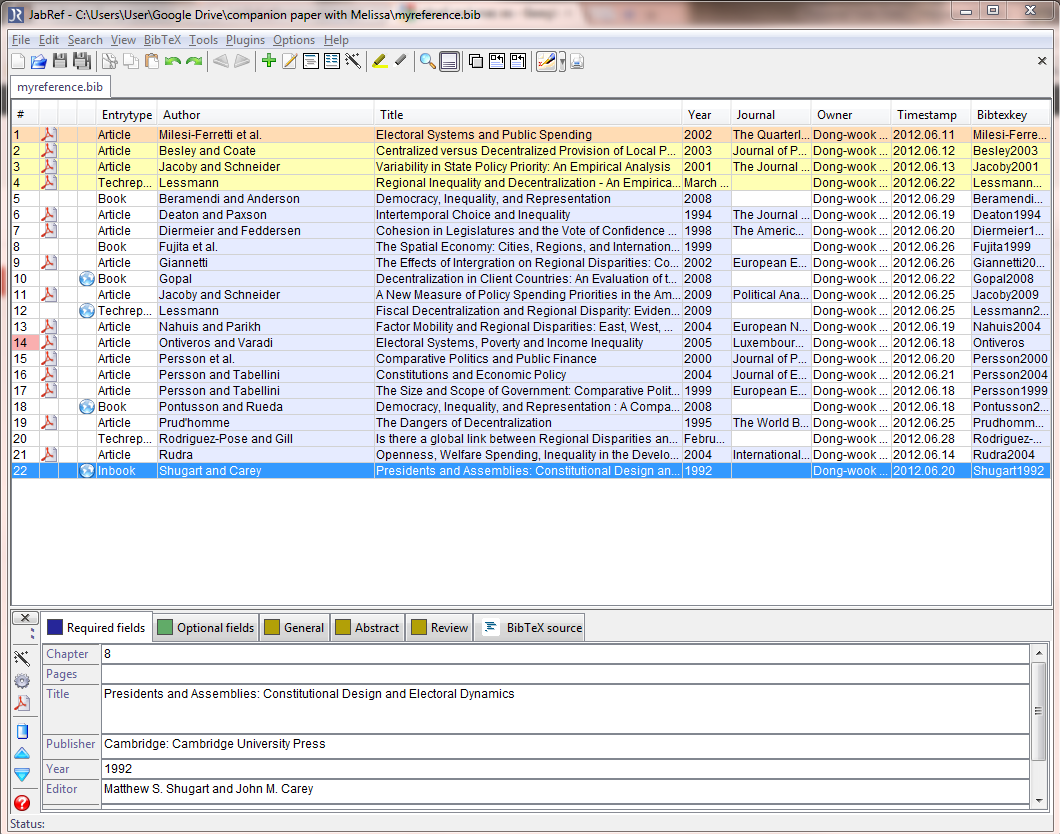
\includegraphics[width=9cm]{img/jabref} % image de X cm de large
%\caption{Titre de la figure} %titre de la figure
%\label{titre_fig} %label de la figure (ex voir figure W)
\end{figure} %fin de l'environnement figure

\vspace*{-0.5cm}
{\footnotesize Téléchargement: http://jabref.sourceforge.net/ }

\end{frame}

%%%%%%%%% SLIDE %%%%%%%%%%%%%%%%%%

\begin{frame}{Mendeley (mutli-plateforme)}

\begin{figure} %debut de l'environnement figure
\centering %figure centree
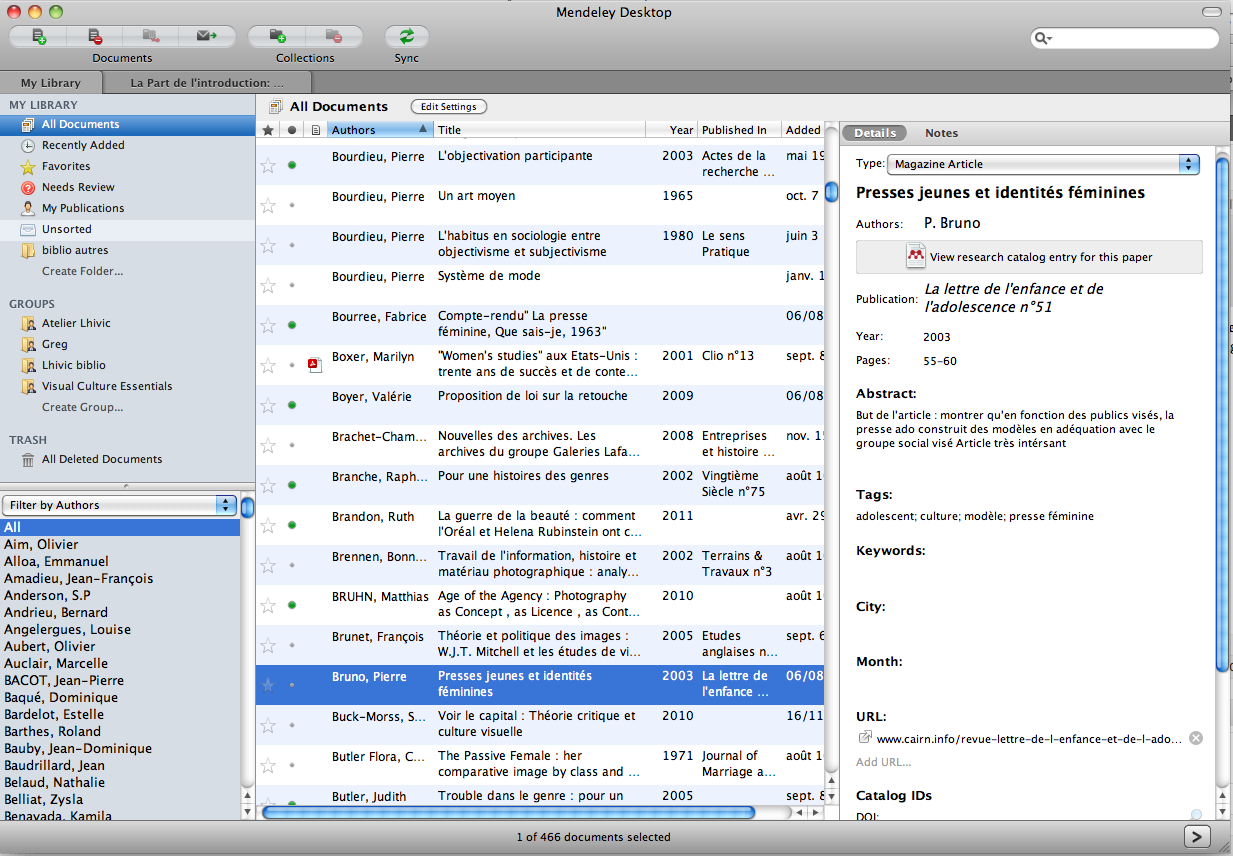
\includegraphics[width=9cm]{img/mendeley} % image de X cm de large
%\caption{Titre de la figure} %titre de la figure
%\label{titre_fig} %label de la figure (ex voir figure W)
\end{figure} %fin de l'environnement figure

{\footnotesize Téléchargement: http://www.mendeley.com/ }

\end{frame}

%%%%%%%%% SLIDE %%%%%%%%%%%%%%%%%%

\begin{frame}{Zotero (mutli-plateforme)}

\begin{figure} %debut de l'environnement figure
\centering %figure centree
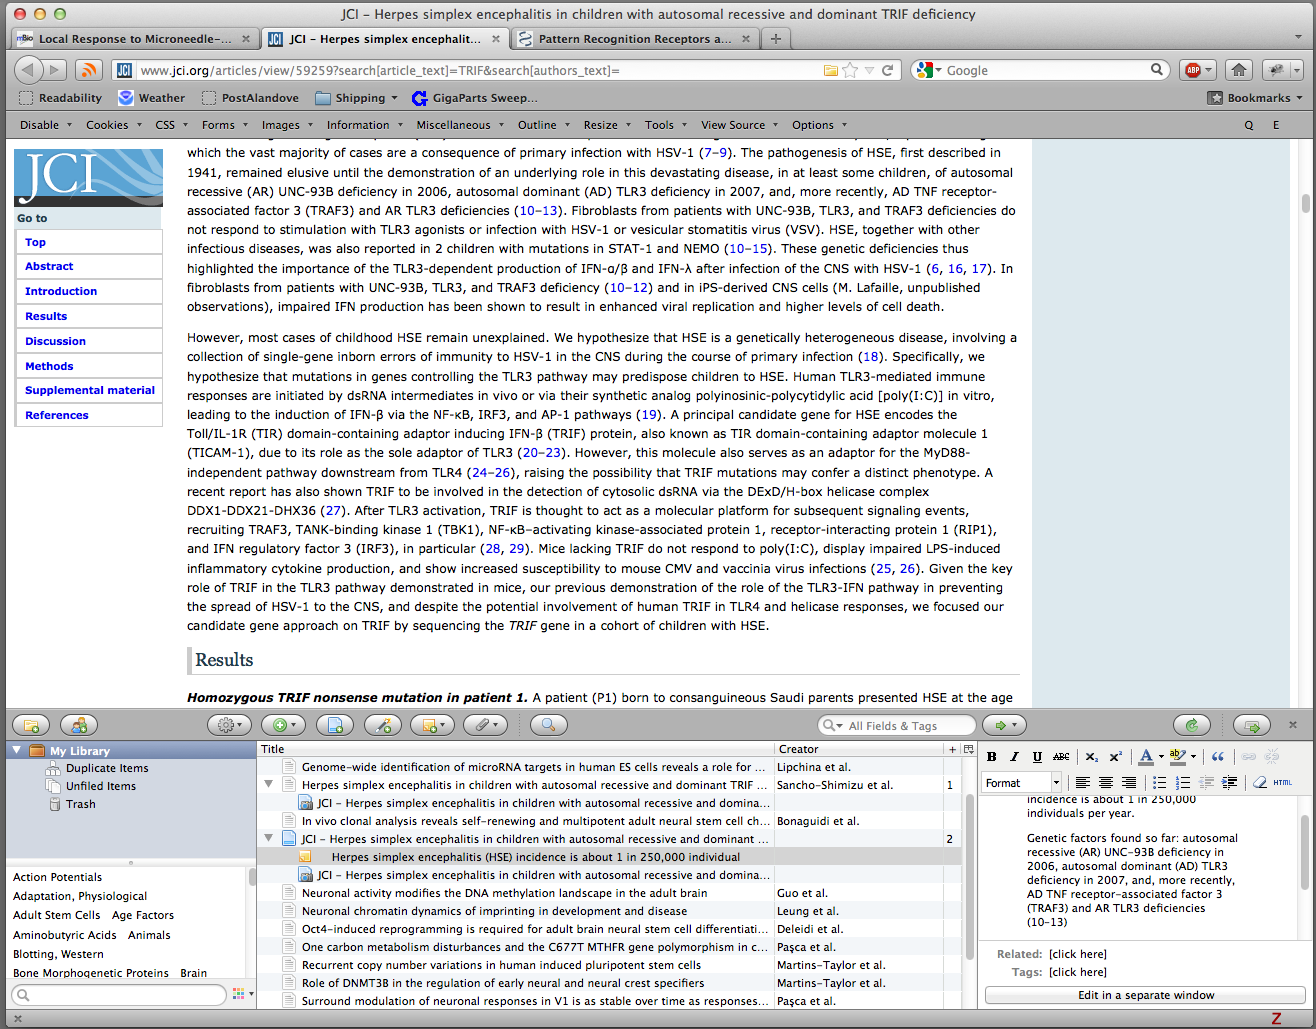
\includegraphics[width=8cm]{img/zotero} % image de X cm de large
%\caption{Titre de la figure} %titre de la figure
%\label{titre_fig} %label de la figure (ex voir figure W)
\end{figure} %fin de l'environnement figure

{\footnotesize Téléchargement: http://www.zotero.org/}

\end{frame}


\begin{frame}
\frametitle{Bibliographie}
\nocite{*} % Bad, should change
\bibliographystyle{abbrv-fr}
\bibliography{latex}
\end{frame}


%%%%%%%%%%
\begin{frame}[fragile]

\vspace*{3mm}

Exercice


\end{frame}

%%%%%%%%%%%%%%%%%%%%%%%%%%%%%%
%%%%%%%%%%% PART%% %%%%%%%%%%%%%%
%%%%%%%%%%%%%%%%%%%%%%%%%%%%%%

\part{Autres éditeurs \LaTeX}


%%%%%%%%% SLIDE %%%%%%%%%%%%%%%%%%

\begin{frame}{Texniccenter}

\begin{figure} %debut de l'environnement figure
\centering %figure centree
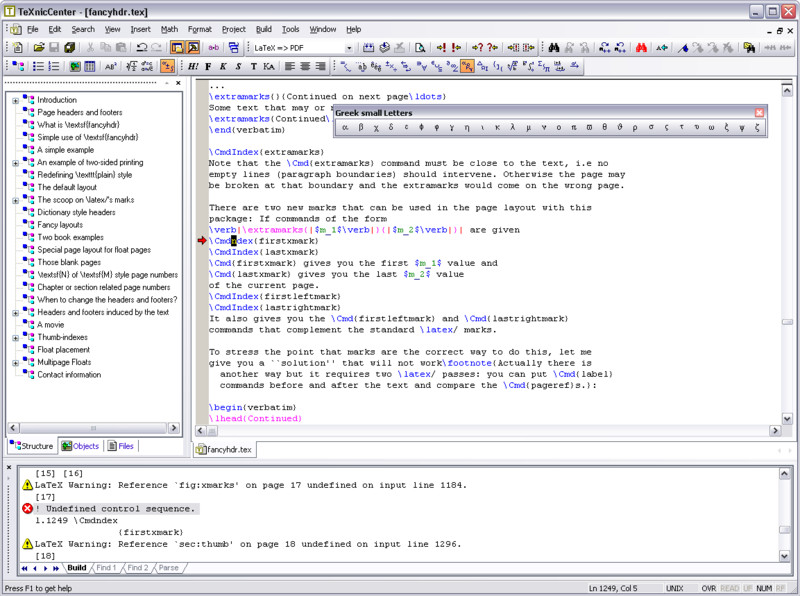
\includegraphics[width=9cm]{img/Texniccenter} % image de X cm de large
%\caption{Titre de la figure} %titre de la figure
%\label{titre_fig} %label de la figure (ex voir figure W)
\end{figure} %fin de l'environnement figure

{\footnotesize Téléchargement: http://www.texniccenter.org/ }

\end{frame}


%%%%%%%%% SLIDE %%%%%%%%%%%%%%%%%%

\begin{frame}{LyX}

\begin{figure} %debut de l'environnement figure
\centering %figure centree
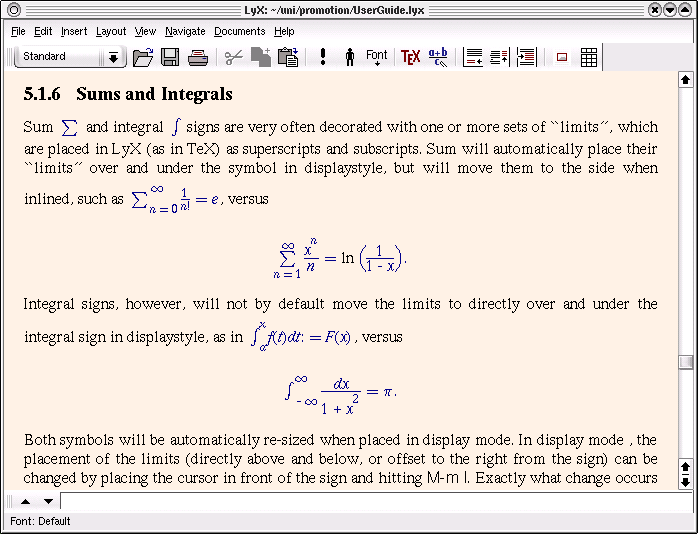
\includegraphics[width=8cm]{img/LyXScreen_Linux_en} % image de X cm de large
%\caption{Titre de la figure} %titre de la figure
%\label{titre_fig} %label de la figure (ex voir figure W)
\end{figure} %fin de l'environnement figure

{\footnotesize Téléchargement: http:// 	www.lyx.org/ }

\end{frame}


%%%%%%%%% SLIDE %%%%%%%%%%%%%%%%%%

\begin{frame}{Texmaker}

\begin{figure} %debut de l'environnement figure
\centering %figure centree
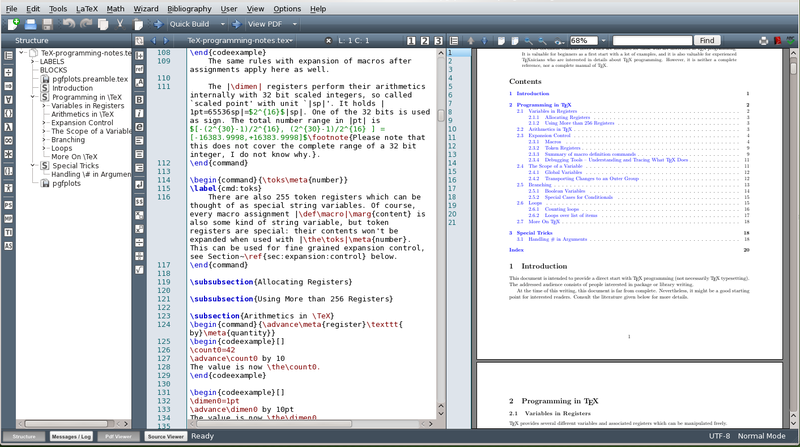
\includegraphics[width=9cm]{img/TexmakerView} % image de X cm de large
%\caption{Titre de la figure} %titre de la figure
%\label{titre_fig} %label de la figure (ex voir figure W)
\end{figure} %fin de l'environnement figure

{\footnotesize Téléchargement: http://www.xm1math.net/texmaker/ }

\end{frame}

%%%%%%%%%%%%%%%%%%%%%%%%%%%%%%%%%%%%%%%%%%%%%%%%%%%%%%%%%%%%%%%%%%%%%%%%%%%%%%%%%%
%%%%%%%%%%%%%%%%%%%%%%%% FIN DU DOCUMENT %%%%%%%%%%%%%%%%%%%%%%%%%%%%%%%%%%%%%%%%%%%%%%%%
%%%%%%%%%%%%%%%%%%% ( NON PRISE EN COMPTE DE LA SUITE ) %%%%%%%%%%%%%%%%%%%%%%%%%%%%%%%%%%%%%%%%%%%
\end{document}
%%%%%%%%%%%%%%%%%%%%%%%%%%%%%%%%%%%%%%%%%%%%%%%%%%%%%%%%%%%%%%%%%%%%%%%%%%%%%%%%%%
%%%%%%%%%%%%%%%%%%%%%%%%%%%%%%%%%%%%%%%%%%%%%%%%%%%%%%%%%%%%%%%%%%%%%%%%%%%%%%%%%%
